\section{Aufgabe 2: Evaluierung von Caching Methoden einer Browser Extension}
\label{s:evaluierungcaching}


\subsection{Speichern von Informationen}
\label{ss:speichern}

Bevor diese Arbeit mögliche Methoden zur Speicherung von Datensätzen evaluiert, werden zuerst grundlegende Fragen beantwortet:

\textbf{Warum benötigt die Extension einen Cache?}:
In Kapitel \ref{ss:aufbauwebsite} zeigt die Abbildung \ref{playstore1} den Aufbau der Internetseite nach bestimmten Themen. Jedes Thema wird mit einer Reihe von Apps dargestellt. Je nach Bildschirmauflösung beinhaltet eine Reihe 7 bis 10 dieser Kacheln.
Beim initialen Aufruf lädt die Seite 8 Themen. Weitere Reihen werden dynamisch beim Scrollen nachgeladen. So findet die Extension zwischen 60 bis 80 App-IDs allein durch den Aufruf der Seite. Wird eine Thema durch den Button \glqq Mehr\grqq{} aufgeklappt, lädt die Seite 120 bis 540 weitere Kacheln. Dabei sind Applikationen oft in mehr als einem Thema vorhanden und bereits auf der Startseite doppelt oder dreifach abgebildet.

Da die Extension pro gefundener App-ID eine Anfrage an das Backend schickt. Entstehen pro Seitenaufruf mindestens 60 und pro Klick auf ein Themengebiet mindestens weitere 120 Anfragen. Also würde ein Nutzer bei einem Besuch der Seite grob geschätzt mehrere hunderte Backend-Anfragen auslösen.

Da diese Webseite als Such- und Einkaufsplattform fungiert, bleibt es in der Regel nicht bei einem einzigen Besuch. Hinzu kommt also eine hohe Redundanz der Anfragen bei erneutem Besuch der Seite. Denn viele Themen und Kategorien, wie zum Beispiel \glqq Empfehlungen für dich \grqq{} sind personalisiert und bleiben über eine Vielzahl an Seitenaufrufen identisch.

Zusammenfassend entstehen bei der Nutzung des Google Play Stores also eine hohe Anzahl an benötigten Informationen mit einer Vielzahl an Redundanz sowohl bei einem Besuch, als auch über mehrere Sitzungen hinweg. Die Veröffentlichung der Extension würde also einen hohes Anfrageaufkommen an das Backend verursachen. Durch eine folgende Überlastung könnte die Extension keine Informationen mehr darstellen und hätte keinen Nutzen mehr.

Der Lösungsansatz ist ein, vom Backend unabhängiger, Speicher, welcher gewonnene Informationen für den Nutzer bereithält. Vor allem langlebige und redundante Daten stehen so ohne wiederholte Anfragen zur Verfügung.


\textbf{Welche Informationen sollen im Cache gespeichert werden?}:
Damit nicht nur die Anzahl der Anfragen an das Backend, sondern auch der Umfang der Daten möglichst gering bleibt, werden die nötigten Informationen und ihrer komprimierten Form angefragt. Dem Backend wird durch bestimmte Parameter signalisiert, nur die Kennzahl der zutreffenden Infobox(siehe Tabellen \ref{tabelleInfofelder} und  \ref{tabelleInfofelderzwei}) zusammen mit der Extraktionsquelle und dem Datum der Extraktion zu der jeweiligen App-ID zu übermitteln.

So entsteht folgender key-value-Datensatz:

\big\{ \textbf{key}: \textit{App-ID}, \textbf{value}: \textit{Extraktionstag in Tagen},\textit{Array von Infoboxen als Zahlen} \big\}

\begin{figure}[ht]
	\centering
	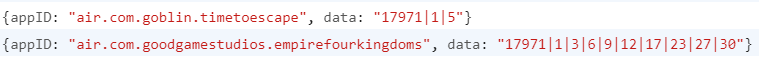
\includegraphics[width=1\textwidth]{pics/cache1.png}
	\caption{Beispiel eines key-value-Datensatzes}
	\label{cache1}
\end{figure}


Die gespeicherten Indizes der Infoboxen werden lokal von der Extension über die Datei \glqq IB\_texte.json \grqq{}(Auszug in Abbildung \ref{cache2}) auf ihre entsprechenden Texte gemappt, sodass diese nicht über das Backend abgefragt werden müssen. Der Extraktionstag dient zur Feststellung des Alters eines Datensatzes. Aktuell ist festgelegt, dass eine Information dann als veraltet gilt, wenn ihr Extraktionsdatum älter als drei Tage ist. Erst sobald die Zeitspanne überschritten wurde, sendet die Extension mit dem nächsten Aufruf der jeweiligen Applikation eine neue Anfrage.


\lstinputlisting[label={cache2},caption={Infobox 19 aus der IB\_texte.json}, firstline=442, lastline=470]{../../Extension/src/lib/data/IB_texte.json}

\textbf{Wie viele Informationen können gespeichert werden?}:
Für die oben gezeigte Struktur der Datensätze ergibt sich folgender \textit{worst-case}:

\textbf{key}: \big\{ \textit{max. 50 characters}\footnote{Gemessen durch Analyse aller App-ID-Einträge während der Evaluation} \big\}

\textbf{value}: \big\{\textit{99999,1,2,3,4,5,6,7,8,9,10,11,12,13,14,15,16,17,}
	
\textit{18,19,20,21,22,23,24,25,26,27,28,29,30,31} \big\}

Das entspricht einer Länge von 50 characters für den key und 89 characters für den value. In UTF-8 sind das umgerechnet ca. 139Byte. Geht man in Google Chrome von einem Limit des Cache-Speichers auf 5200000 characters\footnote{\url{https://arty.name/localstorage.html}} aus, können so ca. 37410 Datensätze gespeichert werden.

\subsection{Kriterien und Vorauswahl}
\label{vorauswahl}

Die Kriterien für eine geeignete Caching-Methode leiten sich aus den Anforderungen aus Kapitel \ref{ss:cacheanforderungen} ab. Zur Auswahl stehen nach Abschnitt \ref{ss:methodeneigenschaften} Cookies, WebSQL, die Web-Storage-API und IndexedDB. Nur Kandidaten, welche alle Kriterien erfüllen werden implementiert darüber hinaus evaluiert.

Die Grundlage für einen geeigneten Cache ist ausreichend Speicherplatz. Während alle anderen Kandidaten mindestens 5MB Speicherplatz zur Verfügung haben, besitzen Cookies mit 4KB Gesamtspeicher pro Domäne, und somit nach der Berechnung in Abschnitt \ref{ss:speichern} mit ca. 28 Datensätzen, zu wenig Speicher für die Extension. 

Das nächste Kriterium ist die Verfügbarkeit. Die Caching-Methode soll uneingeschränkt und überprüfbar zur Verfügung stehen, um die Speicherfunktion der Extension zu garantieren. Aufgrund der genannten EU-Richtlinie in Abschnitt \ref{ss:methodeneigenschaften} und dem Gebrauch von Cookies als Tracking-Methode, beschränken oder blocken viele Nutzer diese Speichermethode. Das stellt eine Ungewissheit dar und widerspricht der uneingeschränkten Nutzung als Kriterium.
WebSQL ist zwar weiterhin in einigen Browsern verfügbar, von einer Implementierung in neue Programme rät der W3C ab\footnote{\url{https://www.w3.org/TR/webdatabase/}}. Durch diese Obsoleszenz erfüllt auch WebSQL das Kriterium nicht. IndexedDB wird als Nachfolger von WebSQL gesehen. Sowohl die Web-Storage-API als auch IndexedDB sind aktuelle Technologien und uneingeschränkt verfügbar.

Abschließend wird der Zugriff auf die Caching-Methoden betrachtet. Der Fokus liegt hier bei einem Zugriff mit möglichst geringer Wartezeit auf viele kleine Datensätze. Alle Kandidaten verfügen über asynchrone Aufrufe, sodass die Extension keine zusätzlichen Wartephasen verursacht. Durch eine fehlende Indexierung verliert die Web-Storage-API jedoch an Performanz, wenn es um das Auslesen von großen Datensätzen geht. Das angestrebte Key-Value-Prinzip wird von IndexedDB und der Web-Storage-API unterstützt. Bei WebSQL erfolgt der Zugrifft über die \glqq Standard Query Language \grqq{} und die Datensätze lägen in Tabellenform vor, was die Handhabung mit den Datensätzen erschwert. Cookies speichern Informationen in Datenobjekte, welche die erwünschten Eigenschaften für den Zugriff ebenfalls erfüllen.

Weder Cookies noch WebSQL qualifizieren sich aufgrund der betrachteten Kriterien als geeignete Caching-Methoden. IndexedDB und die Web-Storage-API kommen beide in Frage und werden in den anschließenden Kapiteln anhand von Messergebnissen und ihren Eigenschaften bei der Implementierung evaluiert.

\subsection{Vorgehensweise}
\label{ss:vorgehensweise}

Die Extension nutzt für die Evaluation den \glqq localStorage \grqq{} der Web-Storage-API, da der \glqq sessionStorage \grqq{} gespeicherte Daten nach Beenden der Sitzung löscht. Die vorgesehene Messung soll Daten über mehrere Sitzungen erfassen. \textit{IndexedDB} wird ohne Framework implementiert.

In drei aufeinanderfolgende Durchläufen werden hier der Aufruf der Website ohne Cache, mit vorhandenem \textit{localStorage} und mit \textit{IndexedDB} verglichen. Die Messung richtet sich nach einer normalen, kurzen Nutzung der Internetseite. Dazu gehört das Laden der Startseite, die Auswahl einer bestimmten Kategorie und das Öffnen einer Detailseite. 

Gemessen wird dieser Prozess mittels der Browser-Konsole von Google Chrome im Reiter \glqq Performance \grqq{}. Dieser ist in der Lage die Ladezeit einer Webseite mit Unterteilung in \textit{Scripting} , \textit{Rendering}, \textit{Painting}, \textit{Other} und \textit{Idle} darzustellen. Die Messung fokussiert sich vor allem die Bereiche \textit{Scripting} und \textit{Rendering} bis zum Ende des \textit{Painting}-Prozesses der Extension. Der zweite Messpunkt sind die Anzahl der Anfragen an das Backend. Diese werden im Reiter \glqq Network \grqq ausgelesen.

Durchführt wurden die Messungen auf der folgenden Plattform:

\begin{table}[h]
	\begin{tabular}{p{4.6cm}R{7.0cm}}
		\toprule
		\textbf{Komponente}	&	\textbf{Eigenschaften/Version}	\\
		\midrule
		Prozessor	&	i7-6700K @ 4.00GHz (8CPUs)	\\
		Speicher	&	16384MB RAM	\\
		Grafik	&	GeForce GTX 1070	\\
		Auflösung	&	2560 x 1440	\\
		\midrule
		Betriebssystem	&	Windows 10 Education 64-Bit-Version (10.0, Build 17134)	\\
		Browser	&	Google Chrome Version 73.0.3683.75 64-Bit	\\
		Internetverbindung	&	Download: 100MBit/s , Upload: 6Mbit/s	\\
		\bottomrule
	\end{tabular}
	\caption{Spezifikationen der Testumgebung}
	\label{cache3}
\end{table}

\subsection{Ergebnisse}
\label{ss:ergebnisseht2}







Storage: none
Ladezeit: 1435ms
Start der Extension-Funktionsaufrufe: 944ms
Dauer: 491ms
Anzahl der Anfragen an das Backend: 0


Storage: Local Storage
Ladezeit: 1711ms
Start der Extension-Funktionsaufrufe: 892ms
Dauer: 819ms
Anzahl der Anfragen an das Backend: 125


Storage: none
Ladezeit: 1761ms
Start der Extension-Funktionsaufrufe: 883ms
Dauer: 878ms
Anzahl der Anfragen an das Backend: 131

IndexedDB: API in allen modernen Browser zur Speicherung von Daten und Dateien in einer object-orientierten Datenbank.
synchron und asynchron möglich.
Funktioniert nach key, value prinzip
Alle Datentypen von JavaScript werden unterstützt.
Kann indexiert werden um Suchen effizient zu machen.
Verwendet Prinzip von Transaktionen
Anfragen mit Rückgabewerten als Basis aller Operationen
Verfolgt den NoSQL-Ansatz

Warum nicht IndexedDB?

Vorteile von IndexedDB: Abspeicherung von großen strukturierten Datenmengen.
Nachteile: hoher Aufwand bei Implementierung.Overhead lohnt nicht bei kleinen Datenmengen. Transaktionen blockieren bei Fehlern  eventuell den Datenabruf bzw. die Aktualisierung

Storage API von Chrome ausreichend Speicher und geringer aufwand bei der Implementierung. Lediglich Strings benötigt. Indices bei gewählen value-Struktur nicht notwendig.

Vorteil von Session Storage: Speicherpflege nicht notwendig, da 5MB groß genug für Anzahl(?) an App-Informationen während einer Session im PlayStore. Informationen immer auf Stand der Quelle
Nachteil: Bei erstmaligen Öffnen des Stores in neuer Browsersession werden viele Anfragen losgeschickt für Apps die bereits in der letzten Session schon angefragt wurden. Bei Serverausfällen fehlen die Informationen
Lediglich in einer Session mehrfach aufgerufene Apps ersparen erneute Anfragen.
=> Speicherpflege fällt weg, dafür kaum Mehrwert bei Anfragen.

Vorteil von Lokal Storage: Apps werden einmal abgefragt und sind anschließend abgespeichert. Fällt der Server aus können die lokalen Informationen genutzt werden. Daten auch aus letzter Session bleiben vorhanden. Neue Anfragen werden nur dann geschickt wenn aktuelle Daten über 3 Tage alt sind.
Nachteile: Speicherpflege notwendig. Dadurch wird die Information länger (Counter und Tag). Zusätzliche Rechenzeit für das Löschen von alten Informationen notwendig. Dadurch wird sichergestellt dass die 5MB nicht überschritten werden und somit Informationen ungewollt verloren gehen. Für Informationen mit hohem Counter muss regelmäßig überprüft werden, ob die Information noch aktuell ist, weil diese in der Regel lange im Speicher verweilt.
=> Hohe Einsparung bei Anfragen an den Server möglich. Dafür müssen zusätzliche Operationen zur Speicherpflege und Prüfung der Informationen ausgeführt werden.


\subsection{Diskussion}
\label{ss:diskussionht2}

Zeitspanne verlängern